\subsection{Image compression}

\subsubsection{Základný náčrt kompresie údajov}
Stratová (ale aj bezstratová) kompresia údajov je založená na
jednoduchých princípoch. Jej hlavné črty si môžeme popísať v troch
krokoch
\begin{itemize}
\item Transformácia
\item Kvantizácia
\item Kompresia
\end{itemize}
Poďme sa bližšie zaoberať jednotlivými časťami.
Transformácia je bezstratová manipulácia s údajmi. Transformáciou môže
byť identita, rozdelenie obrazu na farebné zložky, zmena RGB na CMYK a
pod. Hlavnou úlohou transformácie je akosi predpripraviť dáta na
ďalšie spracovanie, dostať ich do vhodnej podoby pre ďalšie kroky, ale
pritom vedieť stále vypočítať reverznú transformáciu. Krok
transformácie je zároveň krokom, kedy sa nestrácia žiadna informácia.

Nasleduje, druhý krok, samotný krok zodpovedný za stratu informácie
pri stratovej kompresii. Pri bezstratovej kompresii je samozrejme
vynechaný. Výstupom z transformácie sú dáta. Tieto dáta môžeme
považovať za reálne resp. celé čísla. Ich problémom je veľká pamäť
potrebná na udržiavanie týchto informácii. Kvantizácia rieši tento
problém jednoducho inžiniersky - nejaké informácie vynecháme.
Spravidla sa to robí tak, že čísla sa vydelia kvantizačným faktorom a
zaokrúhlia nadol. Opačný proces ku kvantizácii môže len hádať pôvodné
čísla, preto je kvantizácia stratová. Je však na umení príslušného
spôsobu kvantizácie, aké to bude mať vizuálne následky. Ako vieme,
väčšina informácie skrytá v digitálnych obrázkoch či zvukoch je
takpovediac nepotrebná. Človek nemá natoľko vyvynuté zmysly aby ju
všetku videl/počul. Preto záleží len na šikovnosti, ktoré informácie
budú kvantizované viac a ktoré menej. Samozrejme, snahou je najviac
kvantizovať informácie pre človeka skryté a naopak, dôležité údaje
nekvantizovať vôbec. Tu si kvantizácia podáva ruku s predchádzajúcou
transformáciou - čím lepšie transformácia oddelí dôležité od
nedôležitého, tým lepšie vieme kvantizovať.

Poslednou časťou je kompresia. Toto je čiste bezstratová kompresia,
ktorá sa snaží ešte z kvantizovaných údajov vyžmýkať posledné voľné
bity a tak zavŕšiť finálnu podobu.

Príkladom formátu, ktorý nemá transformáciu, nemá kompresiu ale má
kvantizáciu je napríklad bmp - kvantizuje každú farebnú zložku do 8
bitov. Formátom bez transformácie s kvantizáciou a kompresiou môže byť
napríklad tga - prebieha v ňom Run-length kompresia, ktorá vie dobre
komprimovať dlhé úseky rovnakej farby.
V skutočnosti, najviac účinné formáty sú tie, ktoré používajú
sofistikovanú transformáciu. Príkladom je jpeg2000 využívajúci
waveletovú transformáciu či klasický formát jpeg. Práve pri ňom sa
teraz zastavíme a bližšie si popíšeme jeho kroky.

\subsubsection{Jpeg - farebná predpríprava}
Dátový formát jpeg je sofistikovaný formát využívajúci viaceré
poznatky z vizuálneho vnímania obrazu.

V počítači je bežná reprezentácia farieb v takzvanom RGB móde, kde
farba pozostáva z koordinátov v 3D priestore (Červená, Zelená, Modrá).
Hoci je tento spôsob veľmi intuitívny pre CRT monitory, nie je
perfektný pre kompresiu. Trojica farieb červená, zelená a modrá totiž
nepopisuje spôsob vnímania ľudskou bytosťou rovnomerne. Formát jpeg
rieši tento problém zavedením nového farebného priestoru $(Y,Cb,Cr)$,
ktorý sa dá vypočítať nasledovne \footnote{Prevzaté z \ref{jfif}} (predpokladáme 8-bitové RGB hodnoty)
\begin{align}
    Y = 0.299 R + 0.587 G + 0.114 B \\
    Cb = -0.1687R - 0.3313G + 0.5B + 128 \\
    Cr = 0.5R - 0.4187 G - 0.0813B + 128
\end{align}
Pričom spätná transformácia je
\begin{align}
    R = Y + 1.402 (Cr - 128) \\
    G = Y - 0.34414 (Cb-128) - 0.71414 (Cr-128) \\
    B = Y + 1.772 (Cb - 128)
\end{align}
Nasleduje prvá kvantizácia nazývaná Chroma subbampling, 
kde sa zložky  $Cr, Cb$ redukujú na nižšie
rozlíženie. Ľudské oko je totiž omnoho menej citlivé na zmenu farby
ako na zmenu jasu. Pri kompresii si preto môžeme dovoliť zmenšiť
rozlíšenie s akým je uchovaná farba.
Nepríjemným vedľajším dôsledkom môže byť "pretekanie" farebného
odtieňa na silno kontrastných hranách.
\begin{poznamka}
Viac o subsamplingu sa čitateľ môže dozvedieť v 
\todo{wiki}%http://en.wikipedia.org/wiki/Chroma_subsampling}
\ref{subsampling}
\end{poznamka}

\subsection{Jpeg - kosínová transformácia}

Po tejto úprave sa všetky tri vrstvy spracuvávajú samostatne a tým
istým spôsobom. Snahou je zredukovať ďalšiu nepotrebnú informáciu.
Práve tu sa ujíma vedienia Fourierova transformácie, presnejšie
povedané jej kamarátka diskrétna kosínová transformácia. To, prečo je
diskrétna kosínová transformácia výhodnejšia si spomenieme neskôr,
nateraz si vysvetlíme princíp na ktorom zakladajú. Ukazuje sa, že
ľudské oko je vnímavejšie v oblasti nižších frekvencií. Presnejšie
povedané, omnoho viac vnímame svetlosť a odtiene povedzme na veľkej
modrej ploche ako je obloha v porovnaní s rýchlo sa meniacimi farbami
morskej hladiny s vlnami. Diskrétna kosínová transformácia oddelí
jednotlivé frekvencie od seba, a tak môžeme aplikovať rôznu
kvantizáciu pre rôzne frekvencie. Druhou výhodu tejto transformácie je
jej schopnosť sústreďovať väčšinu energie v nízkofrekvenčnej oblasti.
Už bez samotnej kvantizácie vieme potom ušetriť na finálnej kompresii,
ktorá bude omnoho lepšie pracovať na údajoch, ktorých veľká časť má
nízku entropiu oproti vysokej entropii celého pôvodného signálu.
Obraz sa preto rozdelí na bloky veľkosti 8x8 pixelov, každý blok sa
spracúva samostatne.

Na daný blok sa najskôr aplikuje DCT. Výsledok je opäť blok 8x8,
tentoraz vo frekvenčnom spektre. Dáta kvantizujeme pomocou vopred
určenej kvantizačnej matice.

Ukážka prevodu pôvodného obrázku na kvantizované koeficienty a
spätná transformácia je v nasledujúcej tabuľke:


\begin{table}[htb]
    \centering
    \subtable[Pôvodné hodnoty]{
    \tiny
    \input tabulky/informatika/image_compression/original.tbl
    }

    \subtable[DCT]{
    \tiny
    \input tabulky/informatika/image_compression/after_dct.tbl
    }

    \subtable[Kvantizačné koeficienty]{
    \tiny
    \input tabulky/informatika/image_compression/quantization.tbl
    }
    \subtable[Po kvantizácii]{
    \tiny
    \input tabulky/informatika/image_compression/after_quantization.tbl
    }
    
    \subtable[Dekvantizácia]{
    \tiny
    \input tabulky/informatika/image_compression/after_dequantization.tbl
    }
    
    \subtable[Finálny výstup]{
    \tiny
    \input tabulky/informatika/image_compression/final.tbl
    }
    
    \caption{Postupná ukážka kvantizácie JPEG obrázku}
    \label{tab:jpeg}
\end{table}


\subsubsection{Prečo DCT a nie DFT?}
 V krátkosti si vysvetlíme základný rozdiel medzi Fourierovou a
 kosínovou transformáciou pri kompresii. Na prvý pohľad je totiž
 Fourierova transformácia výhodnejšia - ako sme už ukázali, výstup
 diskrétnej Fourierovej transformácie reálnych čísel je zvytočne
 veľký. V skutočnosti, stačí nám $\frac{1}{4}$ výstupu, pretože
 poznáme jeho symetriu v oboch rozmeroch. V spolupráci s predpokladom
 dvojnásobného počtu bitov na zapamätanie si komplexných čísel môžeme
 dôjsť k záveru, že výstup DFT je o polovicu menší ako výstup DCT.
 Tento záver je zjavne v niečom chybný, nakoľko by sme vedeli
 komprimovať ľubovoľné súbory na polovicu. Problém je v  presnosti -
 na výstup DFT potrebujeme väčšiu presnosť aby sme vedeli spraviť
 spätnú transformáciu. Toto ale nie je najhlavnejší dôvod prečo sa
 používa kosínová transformácia.

 Dôvod  prečo DCT a nie DFT si doslova ukážeme.
 Ide o schopnosť koncentrácie energie
 v menších frekvenciách. Z obrázka \ref{fig:dct_vs_dft}
 môžeme vidieť jemný rozdiel medzi týmito dvoma transformáciami
 Fourierova transformácia má najviac koeficientov s väčšou energiou
 ako diskrétna kosínová transformácia. Pri finálnej
 bezstratovej kompresii je to rozhodujúci fakt - kosínová
 transformácia má menej entropie a preto sa bude dať lepšie
 komprimovať.

 
\begin{figure}[htp]
    \centering
    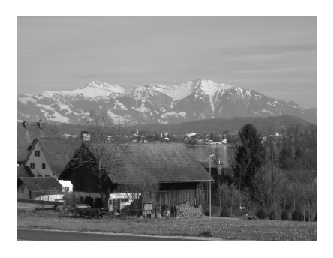
\includegraphics{obrazky/informatika/image_compression/image} \\
    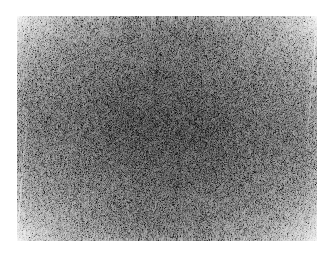
\includegraphics{obrazky/informatika/image_compression/dft}
    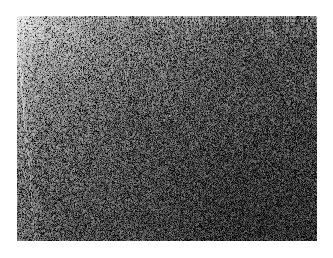
\includegraphics{obrazky/informatika/image_compression/dct} \\
    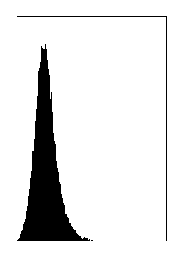
\includegraphics{obrazky/informatika/image_compression/dft_histogram}
    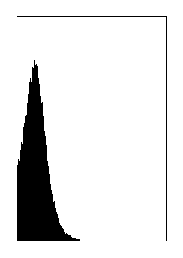
\includegraphics{obrazky/informatika/image_compression/dct_histogram}
    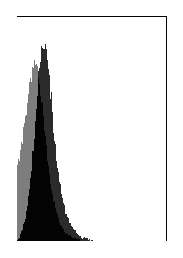
\includegraphics{obrazky/informatika/image_compression/combined_histogram}
    \caption{Porovnanie koncentrácie energie. Vľavo DFT, vpravo DCT,
    obrázok ukazuje normalizáciu koeficientov funkciou $\log 1+|x|$}
    \label{fig:dct_vs_dft}
\end{figure}

\subsubsection{Jpeg kompresia }
\todo{entropy compression}
Nasleduje posledná fáza a tou je kompresia. Kompresia bude fungovať
rôzne pre DC člen (0,0) a zvyšných 63 koeficientov. DC člen spravidla nesie v
sebe väčšinu energie a navyše je známe, že sa veľmi nemení medzi
susednými blokmi 8x8, preto sa počíta ako rozdiel od predchádzajúceho
DC člena. AC koeficienty sa najskôr zoradia do \todo{zig-zag}
postupnosti na obrázku \ref{fig:jpeg_zig_zag}. 

\begin{figure}[htp]
    \centering
    \includegraphics{obrazky/informatika/image_compression/zig_zag}
    \caption{Postupnosť v akej sú kódované AC koeficienty}
    \label{fig:jpeg_zig_zag}
\end{figure}

Zoradenie koeficientov
do tejto postupnosti je pomerne dôležité, pretože empiricky zoraďuje
najskôr najväčšie koeficienty a potom tie menšie až nulové.
Finálna kompresia je \todo{entropy coding}. Jpeg špecifikuje dva možné
pístupy - aritmetické kódovanie a Huffmanovo kódovanie. Aritmetické
kódovanie produkuje o 5-10\% lepšie výsledky, avšak je náročnejšie a
pre rýchle implementácie JPEGu sa používa spravidla Huffmanov kód.

\subsubsection{Ďalšie aspekty JPEGu}

Existuje spústa ďalších aspektov, ktoré sme v tomto krátkom úvode
nespomenuli, a stoja za zmienku. Existuje bezstratová verzia JPEGu,
ktorá funguje na úplne inom princípe. Taktiež, ukladanie dát je možné
rôznymi spôsobmi - sekvenčné a progresívne ukladanie majú každé svoje
výhody. JPEG ako taký môže obsahovať tiež náhľad obrázku, 



\todo{lit: wiki:jfif wiki:jpeg wallace1991}
%
